\documentclass[11pt,twoside,a4paper]{article}
\usepackage{graphicx}
\usepackage{amsmath}
\usepackage{mathrsfs}
\usepackage{graphicx}
\usepackage{float}
\usepackage[parfill]{parskip}
\usepackage{listings}


\begin{document}
\lstset{
   basicstyle=\fontsize{8}{9}\selectfont\ttfamily}
\setcounter{secnumdepth}{4}
\title{M4R}
\author{Anthony Webster CID 01051827}
\maketitle
\clearpage
\section{Abstract}
The aim of this project is to build on previous research and develop an efficient steady Navier-Stokes solver. Utilizing a Lagragian preconditioner described by Patrick et al in \textit{An Augmented Lagrangian Preconditioner For The 3D Stationary Incompressible Navier–Stokes Equation At High Reynolds Number}, the grad-div stabilization method described by Olshanskii et al in \textit{Grad-div stabilization for Stokes equations} and the BDM/DG discretization of the $H_{div}$ space we derived a weak form of the Navier-Stokes Equation and obtained from it a working Stokes and Navier-Stokes solver.\\
The primary advantage of the $H_{div}$ space is that the divergence free requirement of the continuity equation is satisfied exactly globally. This allows the Schur Complement to be exactly determined rather than approximated as in Patrick et al's paper.
We then noticed that at high Reynolds number the Navier-Stokes solver tended to fail. Hence we developed a continuation method which decreases computational cost and extends the Reynolds number for which the solver works.\\
We demonstrated all of the above in various test cases. \\
Finally we gave a summary of possible future improvements.
\clearpage

\tableofcontents
\clearpage

\section{Introduction}
The steady Navier-Stokes equations govern steady state fluid interactions. These may arise due to lack of significant temporal changes of a system. One of the primary motivations of study is whether or not these form stable steady solutions to the full Navier-Stokes equations. In this context this project provides the base flows on which the stability analysis would then be performed. Examples of particular interest of steady flows are pipe flows and flows past a cylinder. The latter has interesting properties, which display fundamental mechanisms, and its industrial applications [14].\\
We seek to create an efficient solver of the steady Navier-Stokes equations in an arbitrary domain. For this the Finite Element method is particularly suited, and has been used for this purpose in the past [20]. \\
Recent papers [2,9] have demonstrated the use of a modified Schur preconditioner along with a grad-div stabilization method to be highly efficient. We seek to combine this with a discretization in a globally divergence free [18] space. This allows us to exactly get the Schur complement mentioned in [2], as it will lie in the $H_{div}$ space, rather than approximating it.\\
\\
The steady Navier-Stokes equations are as follows :
\begin{align}
(u \cdot \nabla) u &= -\nabla p + \mu \nabla^2 u + F \\
\nabla \cdot u &= 0
\end{align}
First we will describe the classic continuous Galerkin (CG) finite element method, its advantages and disadvantages, hence explaining why we are using a modified method. Next we will explain a number of definitions and tools used in the project and which may be unfamiliar to some readers. Then we will show how to find the weak form of the equations and build different parts of our solvers. Finally we will consider some example cases and test whether the algorithm converges to the right result at satisfactory rates.\\

\section{Tools and Definitions}
A number of well-known methods, algorithms and definitions are used in this report. This section serves to quickly introduce these concepts for latter use. We will first start by explaining the general finite element method, specifically the most commonly used continuous Galerkin method. We then will explain Newton's method for non-linear matrix equations which arise from the finite element discretization of the Navier-Stokes equation. Then we explain the general concept of preconditioners. Lastly we will define the various notations involved in this project.

\subsection{Continuous Gelrkin Finite Elements Method}
The Finite Element Method (FEM) is a numerical method which approximates the solution to an exact partial differential equation [5]. One of the reasons it is widely used in research, industry and in this project is because it works on arbitrary domains. This is preferable to the finite difference method, which finds exact solutions to an approximated discretized partial differential equation.\\
We will now consider the case of applying the FEM to the Stokes equations using the more common continuous Galerkin method. We do this to explain how conventionally this problem would have been solved, and how our method will improve on it.\\
This method in particular is very common in research and for industrial problems. As such there are a number of courses and books on the subject, such as \textit{Galerkin finite element methods for parabolic problems} [6] if further explanation and theory is required.\\
\\
The Stokes equation is :
\begin{align}
0 &= -\nabla p + \mu \nabla^2 u + F \\
\nabla \cdot u &= 0
\end{align}
As seen in Common and Unusual Finite Elements [7], the Lagrange finite element used in CG approximates a function on a cell using polynomials of degree $q$, defined by their pointwise values at an array of points. Maximal global continuity is kept by making sure that multiple cells agree on their respective edges.\\
For instance let us approximate $f = \sin(x)$ from $0$ to $2 \pi$ using 1D first order Lagrange finite elements. We approximate the function on each of the four cells by a linear function. This linear function is defined on each cell using two points in it, the two edge points. Hence we get figure 1, where the blue curve indicates our approximation and the red one the exact function. In practice one can consider $f$ to be the sum of these linear functions. Note that this element is continuous across the "edges" of a cell, since regardless of the cell, the value of the interpolated function at the "edge" will be identical. This concept can be extended to 2D.\\
\begin{figure}
  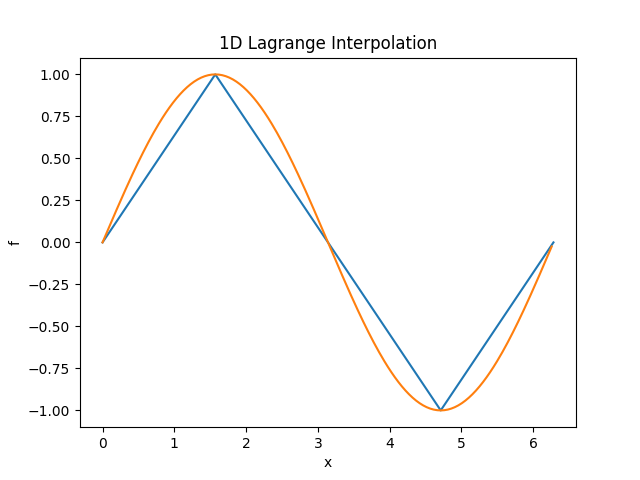
\includegraphics[width=\linewidth]{ex_1D_LG.png}
  \caption{4 Element First Order Interpolation Example and Comparison to True Solution}
\end{figure}
\\
We cut up our domain into a mesh. Commonly these meshes are made up of triangles for simplicity, although squares or even curved elements, for simulations on a sphere, are also used. These elements form the cells. Then we approximate $u$ and $p$ using the Lagrange element in each cell. Hence we get that for instance $u$ is the sum of a set of known piecewise linear functions (as they are determined by the mesh) but with unknown coefficients. The aim of the rest of the method is to determine these unknown coefficients.\\
For that end we need to find what is called the weak form of the equation. We multiply (3) by an arbitrary function $v$. Hence we get :
\begin{align*}
\int_{\Omega} -v \cdot \nabla p + \mu v \cdot \nabla^2 u dx = -\int_{\Omega} v \cdot F dx .
\end{align*}
Since our domain $\Omega$ is cut out into triangles we can cut the integral into triangles and work on each one individually. Hence for each cell $e$ in $\Omega$ we get,
\begin{align*}
\int_{e} p \nabla \cdot v + \mu v \cdot \nabla^2 u dx =  -\int_{e} v \cdot F dx .
\end{align*}
However since $u$ and $v$ will be approximated by functions which may be discontinuous in their derivatives, $\nabla^2$ may not be defined. We then proceed by integration by parts,
\begin{align*}
\int_{e} p \nabla \cdot v - \mu \nabla v \cdot \nabla u dx = -\int_{e} v \cdot F dx .
\end{align*}
Finally multiplying (4) by a similar pressure test function $q$ and adding it to the left hand side of the above we get :
\begin{align}
\int_{e} p \nabla \cdot v - \mu \nabla v \cdot \nabla u dx + \int_{e} q \nabla \cdot u dx = -\int_{e} v \cdot F dx .
\end{align}
Now we use the fact that $q$, $v$, $F$, $u$ and $p$ are a sum of known linear functions and coefficients.\\
Pulling out and removing the coefficients of $v$ we get that :
\begin{align*}
 \int_{e} \sum_i \sum_j (  p_j \phi_j \nabla  \cdot \Phi_i - \mu \nabla \Phi_i \cdot u_j \nabla \Phi_j +   \phi_i u_j \nabla \Phi_j) dx = -\int_{e} \sum_i \Phi_i \cdot F_i \Phi_i dx .
\end{align*}
Combining all the triangles we can eventually turn our problem into a matrix equation of the following form,
\begin{align}
M x = b ,
\end{align}
where $x$ is a vector of coefficients of $u$ and $p$.\\
We can solve this using a variety of linear systems solvers. Note in particular that the majority of basis functions, $\Phi$ and $\phi$, are $0$ in any given triangle, therefore the matrix $M$ will be sparse.\\
While we locally enforced the divergence-free equation by including it in the weak form, the global flow may not be divergence-free. In order to achieve that more complex mathematical tools would be required.\\
Now apply this to the manufactured solution :
\begin{align*}
u_x =  &-\sin(2 \pi y)^5 \cos(2 \pi y)  \sin(2 \pi x)^6, \\
u_y = &\sin(2 \pi x)^5 \cos(2 \pi x)  \sin(2 \pi y)^6, \\
p = &10^{-2} \sin(2 \pi x)^2 \sin(2 \pi y)^2, \\
F_x =& -(2 \pi \cdot 10^{-2} \cdot \sin( 2 \pi x) \cos(2 \pi x) \sin(2 \pi y)^2 \\
	&- 8 \pi^2 \sin(2 \pi x)^4 \sin(2 \pi y)^3 \cos(2 \pi y)(-11 \sin(2 \pi x)^2 \sin(2 \pi y)^2 + 10 \sin(2 \pi x)^2 \cos(2 \pi y)^2 \\
	& + 15 \cos(2 \pi x)^2 \sin(2 \pi y)^2 )),\\
F_y = &-(2 \pi \cdot 10^{-2} \cdot \sin( 2 \pi y) \cos(2 \pi y) \sin(2 \pi x)^2 \\
	&+ 8 \pi^2 \sin(2 \pi y)^4 \sin(2 \pi x)^3 \cos(2 \pi x)(-11 \sin(2 \pi y)^2 \sin(2 \pi x)^2 + 10 \sin(2 \pi y)^2 \cos(2 \pi x)^2 \\
	&+ 15 \cos(2 \pi y)^2 \sin(2 \pi x)^2 )).
\end{align*}
$F$ was selected specifically to ensure that any given $u$ and $p$ are solutions. We can verify this by checking that $F = \nabla p - \nabla^2 u$.
Using the above and implementing a solver using CG2 and CG1 in firedrake we get figures 2 and 3. On a mesh with 64x64 vertices we get an error of $10^{-11}$ for velocity and $10^{-10}$ for pressure.\\
However, default implementation using the CG method is slow, hence we wish to improve on it.\\
Additionally we had to modify our problem for the solver to converge at all. When we increased the order of magnitude of $p$ (and adjusted $F_x$ and $F_y$ accordingly) the solver failed in tests. It is likely that the CG solver described failed due to these terms making the matrix equation ill-behaved  when attempting LU factorization.
\begin{figure}
  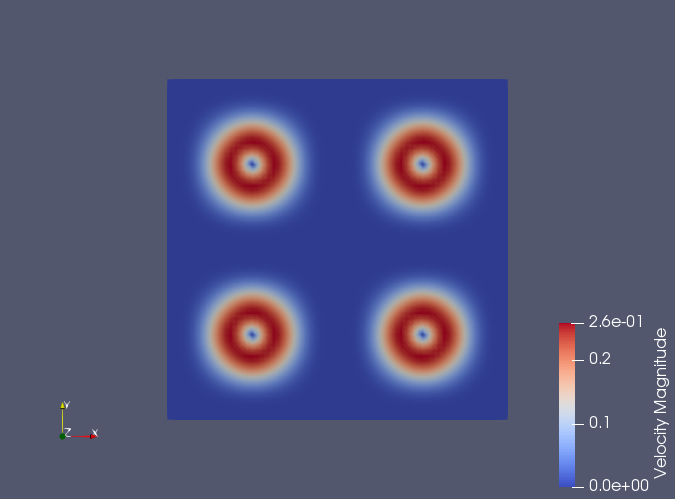
\includegraphics[width=\linewidth]{lgv.png}
  \caption{Standard velocity CG solution in a 64x64 vertex uniform square. We obtained a velocity error of order $10^{-11}$.}
\end{figure}
\begin{figure}
  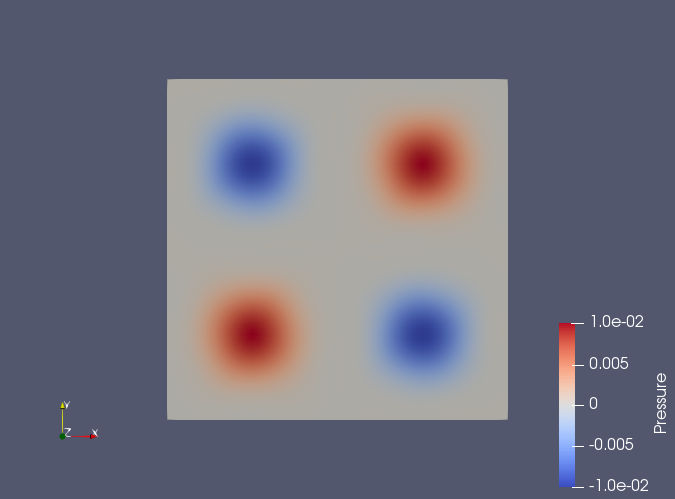
\includegraphics[width=\linewidth]{lgp.png}
  \caption{Standard pressure CG solution in a 64x64 vertex uniform square. We obtained a pressure error of order $10^{-10}$.}
\end{figure}

\subsection{BDM-DG Mixed Space}
Let us introduce the mixed space we will be working in for the rest of the paper. We will first define Brezzi-Douglas-Marini and explain the restrictions that come with it, then the discontinuous Galerkin and how, combined with the BDM element, we have an $H_{div}$ space.\\
\\
The paper Common and Unusual Finite Elements [7] states that the BDM space on one triangle $K$ is composed by polynomials of order $q$ defined by the normal component on each edge. If $q > 1$ it is also defined using the integration against gradients of the polynomials on the triangle. If $q > 2$ we then also use the integration  against curls of $b_K P_{q-2}(K)$ where $b_{q-2}$ is the cubic bubble function associated with $K$ and $P_{q}(K)$ is the set of polynomials defined on $K$.\\

However unlike the Lagrange elements we can no longer set a Dirichelet boundary condition's tangential component. Therefore we need to find alternative approaches to enforce these conditions, such as boundary penalty methods as seen in [21] and [22].
Additionally some operations (such as the weak form of the curl) are undefined in this space. Due to possible discontinuities at the boundaries we have to be careful with all boundary integrals.
In general the weak form will be far more complex.\\
\\

The discontinuous Galerkin Element space is the space of piecewise linear discontinuous functions. An example applying this space on its own can be found in [8].\\
This finite element, combined with the BDM element for velocity, discretizes the function space $H_{div}$. A property we thus get from simply working in the BDM/DG mixed space is that our solution will be exactly divergence free globally and locally.
Additionally we will be able to more efficiently employ an enhanced Lagrangian preconditioner thanks to the global divergence free property [2].\\

\subsection{Newton's Method}
The Navier-Stokes equations have a non-linear part in the advection term for the velocity component. Hence we will need an algorithm to solve non-linear equations. We will thus describe Newton's method in this section.\\
\\
Consider the non-linear equation of the form :
$$
F(x) = 0 ,
$$
where $F$ is a vector function and $x$ is vector of unknowns. Note that $F$ may be non-linear and have constant components.
For instance we could have $ F = x^T A x + M x - b$, where A and M are constant matrices and b is a constant vector.\\
We start with a guess $x = x_0$ and then determine the Jacobian of $F(x)$, call it $DF(x)$.\\
We determine the Jacobian by calculating the Gateaux derivative, defined as follows [12] :
\begin{align}
DF_{x_n}(\Delta x) = lim_{t \rightarrow 0^+} \frac{F(x_n+ \epsilon \Delta x) - F(x_n)}{\epsilon}.
\end{align}
We then use the vector Taylor expansion :
\begin{align*}
F(x_{n+1}) = F(x_n) + DF_{x_n}(\Delta x) \Delta x.
\end{align*}
Hence we get the algorithm :
\begin{align}
DF_{x_n}(\Delta x) \Delta x = - F(x_n) ,\\
x_{n+1} = x_n + \Delta x.
\end{align}
We solve for $\Delta x$ using $x_n$ and the Taylor expansion approximation and then use this result to determine $x_{n+1}$.
This is a linear problem which can be solved via an LU Factorization for instance.\\
Note that the Newton's method only converges and is unique if it is within a ball around the solution [10-11]. Other methods may be required to get to that point.

\subsection{Preconditioners}
Computational cost of an algorithm is an important limitation which we want to reduce as much as possible. This is especially true given that many experimental and industrial applications will require very high resolution to take into account the complex shapes and boundary layers involved. As such we utilized a Schur preconditioner to keep the computational costs down. This section will introduce the general concept of preconditioners. What is briefly discussed here can be found in further detail in the book Multilevel Block Factorization Preconditioners [4] on pages 49 to 51.\\
\\
Take the system :\\
$$
Mx = b ,
$$
where $M$ is a very large matrix, assumed for simplicity to be symmetric, $x$ an unknown vector we need to solve for (in our case this will be a vector of coefficients for both $u$ and $p$) and $b$ a constant vector (containing forcing and boundary conditions for our problem). If $M$ is a symmetric positive definite sparse matrix then $M$ applied to a vector is cheap to compute. Hence we can easily find $r$, the residual.\\
$$
r = b - Mx .
$$
We then use the resulting $r$ in order to provide a correction on our result.\\
However $M$ may not be well-behaved. In fact in our problem we know it is usually not, since it is an elliptic problem.\\
In this case we use a preconditioning matrix $P$, to map the system in such a way that $P^{-1}$ is cheap to compute, this operation can easily be parallelized and the condition number, the ratio of largest and smallest eigenvalue which describes the behavior of the system [13], is lowered (this implies better numerical behavior).\\
We then numerically solve the transformed and, usually, better behaved system :
$$
P^{-1}(Mx-b) = 0 .
$$
This procedure allows us to transform a computationally ill-behaved matrix equation (unstable, non-sparse, etc.) into an easier one.

\subsection{Notation}
Various notations are used throughout this paper. Although they are fairly common amongst papers in the subject we will re-introduce them here. Additionally this will allow us to explain some concepts which may not be familiar to some readers.\\
\\
$\Omega$ is the computational domain we are working on (this may be the unit square or an annulus for instance).\\
\\
$\partial \Omega$ denotes the boundary of that domain.\\
\\
$e$ denotes an individual triangle composing the mesh which forms $\Omega$. In this context $\sum_e$ denotes a sum over all triangles of the mesh.\\
\\
$\Gamma$ denotes the boundary of an individual triangle $e$.\\
\\
Let us define $a_+$ and $a_-$.\\
When the mesh is setup we ensure each facet (ie. edge of a triangle) in the mesh has a positive and negative side, and each cell agrees on which is which. We call these terms on facet integrals. Then $a_+$ is the value of $a$ on the positive side $a_-$ on the negative side. The normal usually points from the negative to the positive side. However, when we consider for instance $(n \cdot a)_+$ we consider the whole expression on the "positive side" including the normal, which, with respect to any given cell, always points out of the cell, and hence may point in the opposite direction of the standard normal of the facet.\\
It is important to note that the positive and negative side are completely arbitrary. They serve as markers for the method. Obviously these terms do not appear in the continuous finite element spaces.\\
For facets which are facing the exterior domain we usually consider the equations separately.\\
\\
Let $\{ a \} = a_+ + a_-$. \\
This is a summation term. Due to discontinuities of our space on facet elements integrals over facets from integration by parts on an individual element will not disappear necessarily, hence these terms remain. Additionally, since we cannot use Dirichelet boundary conditions, weak penalty terms will also use this operation.\\
For integrals over the outer facets we explicitly write out the formula for clarity.\\
\\
Let $J(a) = a_+ - a_-$\\
This is a jump term. Note that this operation is $0$ in a continuous space, which is where we assume the physical fluid velocity and pressure to be.\\
\\
We may have surface integrals over interior facet and exterior facet, which are on the computational boundaries.\\
In the first case the integral of $a$ is $\int_\Gamma a dS$ while in the latter we note $\int_{\delta \Omega} a ds$.\\
This is used both for additional clarity and because it is the notation in the code.\\
\\
sgn(k) is the sign of scalar k.

\section{$H_{div}$ Solver}
This section will explain the solver setup of the Navier-Stokes Equation. First we will deal with discretizing the steady Stokes equation, which is linear, and explain how to implement the modified Schur complement to improve performance. Then we will move on to the steady Navier-Stokes, first finding the weak form of the advection before introducing the continuation method. Lastly we will discuss a time stepping solver for the unsteady Navier-Stokes in order to study stability of solutions obtained from prior methods.
\subsection{Steady Stokes}
The linear nature of the Stokes equation makes it easier to solve, hence we considered it first. We will start from the strong form of the Stokes Equation and find a weak form. Then we will explain the modified Schur preconditioner.\\
The following is the standard strong form of the Stokes equation.
\begin{align}
0 &= -\nabla p + \mu \nabla^2 u + F , \\
\nabla \cdot u &= 0 . \nonumber
\end{align}

\subsubsection{Weak Stokes Equation}
In this section we aim to find the weak form of the steady Stokes equation, required for building the matrix system as seen in the classic FEM.\\
We start off by cutting our computational domain $\Omega$ into a set of cells $e$. As discussed above it is now required to find the weak form of equations (9) and (10) in the BDM/DG space.
For this purpose let us introduce two test functions, $w$ in BDM for velocity and $q$ in DG for pressure.
Let us multiply equation (9) by $v$ and integrate over the domain as seen in the first section.
\begin{align*}
\int_\Omega v \cdot F dx &= \int_\Omega (v \cdot \nabla p) dx - \int_\Omega (\mu v \cdot \nabla^2 u) dx .
\end{align*}

Again we can work on each cell $e$ individually and then sum it all up.
\begin{align*}
\sum_e \int_e v \cdot F dx &= \sum_e (\int_e (v \cdot \nabla p) dx - \int_e (\mu v \cdot \nabla^2 u) dx) .
\end{align*}
Focusing on the viscosity, or second, term we obtain via integration by parts:
\begin{align*}
\int_e (v \cdot \nabla^2 u) dx = - \int_e \nabla_h(v) : \nabla_h(u) dx + \int_\Gamma 2 \{ v_i n_j \} \{ \frac{\partial u_i}{\partial x_j}\} dS .
\end{align*}
The first term can be summed up to an integral over $\Omega$ and the second one is asymmetrical. We can add a term to make it symmetrical. This helps with numerical stability of the final matrix equation. Numerical stability ensures that if there are errors in the input values of the problem (such as the exact values of an inflow), they lessen as the algorithm progresses. This property is obviously desirable especially when considering experimental information. Most measurement devices have a certain tolerance below which the measured value is uncertain. Additionally some linear solvers take advantage of this structure.\\
Hence we proceed to get :
\begin{align*}
-  \int_\Omega \nabla_h(v) : \nabla_h(u) dx + \sum_e( \int_\Gamma 2 \{ v_i n_j \} \{ \frac{\partial u_i}{\partial x_j}\} dS + \int_\Gamma 2 \{ u_i n_j \} \{ \frac{\partial v_i}{\partial x_j}\} dS) .
\end{align*}
Our physical velocity field is presumably continuous.
So $u$ should be continuous in the physical space thus the added term will be $0$ in continuous space. Hence this does not change the equation in physical space as added terms amount to $0$ physically.\\
\\
Now we also add the term $\alpha \int_\Gamma \frac{1}{h}  J(v_i) J(u_i) dS$. According to sources [3] and testing provided that  $\alpha$ is larger than $10$, numerical stability is increased.
($J$ is the jump notation described in 3.5).\\
The numerical value of $h$ is the average distance of a side. In our case we defined it as the average cell-volume over the length of the facets between them for each individual facet element $\Gamma$.\\
Again, any flow studied with this algorithm will have a continuous velocity and pressure fields. The $J(u_i)$ term makes this integral $0$ in continuous space so this does not change the equation.\\
\\
As mentioned in section 3.2, we cannot set the tangential component of a Dirichelet boundary condition in the conventional manner.  So instead we include the boundary conditions in the weak form as a forcing term. These push the solution towards respecting the boundary conditions. In practice this means that when considering the edge integrals for facets facing the exterior of the domain, we set $u$ equal to the Dirichelet boundary condition there.\\
 Hence our final viscous term becomes :\\
\begin{align*}
&-  \int_\Omega \nabla_h(v) : \nabla_h(u) dx + \sum_e ( \int_\Gamma 2 \{ v_i n_j \} \{ \frac{\partial u_i}{\partial x_j}\} dS + \int_\Gamma 2 \{ u_i n_j \} \{ \frac{\partial v_i}{\partial x_j}\} dS, \\
&- \alpha \int_\Gamma \frac{1}{h}  J(v_i) J(u_i) dS \ ) + \int_{\partial  \Omega} v_i n_j \frac{\partial(u_i + u^0_i)}{\partial x_j} + (u_i + u^0_i) n_j\frac{\partial v_i}{\partial x_j} ds - \alpha \int_{\partial \Omega} \frac{1}{h} v_i(u_i-u^0_i)ds .
\end{align*}
Where $u^0_i$ are the boundary values.
We will call this term $\eta_\mu$ for ease of writing.\\
We then return to our original equation with the term above.
\begin{align}
\int_\Omega v \cdot F dx &= \int_\Omega v \cdot \nabla p dx - \eta_\mu .
\end{align}
Let us consider the continuity equation again :
\begin{align*}
\nabla \cdot u = 0 .
\end{align*}
Multiplying by $q$ and integrating we get :
\begin{align*}
\int_\Omega q \nabla \cdot u dx = 0 .
\end{align*}
This is $0$, so we add this to the weak formulation $(11)$ we obtained, getting one weak formulation which includes both pressure and velocity while also keeping symmetry. As seen in the appendix this is required to the usage of a mixed space in UFL.\\
We need this since we want to turn the entire system into a single matrix equation which includes all the conditions. Since we are working the the $H_{div}$ space and the solution to the continuity equation is in $H_{div}$ we just ensured that the velocity will be divergence free globally.\\
We integrate the pressure term by parts in $(11)$ and add the continuity equation we obtained.
\begin{align}
\int_\Omega v \cdot F dx &= \int_{\partial \Omega p} \ v \cdot n ds - \int_\Omega  p ( \nabla \cdot v) dx + \int_\Omega q (\nabla \cdot u) dx  - \eta_\mu .
\end{align}
But v is $0$ on all the boundaries, hence we get :
\begin{align}
\int_\Omega v \cdot F dx &= - \int_\Omega  p ( \nabla \cdot v) dx + \int_\Omega q (\nabla \cdot u) dx  - \eta_\mu .
\end{align}

\subsubsection{Schur Preconditioner}
In an effort to get our iteration count to be independent of mesh-size, we will apply a Schur preconditioner similarly described in chapter 3 of Multilevel Block Factorization Preconditioners [4] and applied to our problem in [2] and [9]. This will dramatically reduce the computational cost of the solver.\\
This is a well-known method. However, as we will be modifying it, we will quickly describe it as well.
Our system effectively amounts to solving a matrix equation of the form :
$$
\begin{bmatrix}
A         & B^{T}\\
B         & 0 \\
\end{bmatrix}
\begin{bmatrix}
u    \\
p     \\
\end{bmatrix}
=
\begin{bmatrix}
b    \\
0     \\
\end{bmatrix} ,
$$
where $B$ is the discretized divergence operator and $B^T$ the discrete gradient operator. $A$ contains the viscous term.
Setting $S = - B A^{-1} B^{T}$, we can factorize the above and get an expression whose inverse is :
$$
\begin{bmatrix}
I         & - A^{-1} B^{T}\\
0         & I \\
\end{bmatrix}
\begin{bmatrix}
A^{-1}   & 0\\
0       & S^{-1} \\
\end{bmatrix}
\begin{bmatrix}
I & 0\\
 - B A^{-1}       & I \\
\end{bmatrix} .
$$
Hence, if we can find $A^{-1}$ and $S^{-1}$ we can easily solve the equation.\\
We solve for $A^{-1}$ or, to be exact, the operation $A^{-1}v$ via an LU factorization. The LU factorization is a direct solver, and thus is inefficient. The algorithm would have to be performed in a sequential manner, preventing usage of parallelization. We did mitigate this through the usage of the "mumps" sub-routine. We originally attempted to use ILU, which is more efficient, but this failed. This is a consequence of the approximation of the Schur complement we will now describe.\\
 $S^{-1}$, the inverse of the Schur complement is difficult to determine because it is usually dense. However research has shown [2 \& 9] that we can solve this issue by using a "grad-div" stabilization method. We add the term $\gamma \nabla \cdot v \: \nabla \cdot w$ to equation (13). Note that this term is 0 if the terms were continuous, as they should be physically.
\begin{align}
\int_\Omega w \cdot F dx &= \int_\Omega \nabla \cdot (p v) dx - \int_\Omega ( p \nabla \cdot (v)) dx - \int_\Omega q (\nabla \cdot u) dx  - \eta_\mu + \int_\Omega \gamma \nabla \cdot u \: \nabla \cdot v dx .
\end{align}
This doesn't change the equation, thus should result in the same solution. However according to the same papers [2 \& 9] we can then approximate $S$ by the pressure mass matrix. Due to the fact that the pressure mass matrix is block diagonal we can easily invert it to find $S^{-1}$.
\\
Note that in theory we could have tried a similar method in the CG space.
Testing shows however that this fails.
This makes sense as we utilized the exact divergence free-property of our space for the Schur complement. One could consider that we used the continuity equation to reduce the system to a single equation, which doesn't hold if velocity isn't globally divergence-free.
As a result in the CG space, as gamma tends to infinity, S does not exactly tend to the pressure mass matrix.\\
This obviously makes our assumption invalid and finding $S^{-1}$ considerably harder.

\subsection{Steady Navier-Stokes}
We now have a discretization of the steady Stokes equation and an efficient Preconditioner for it.
Our aim is to solve the steady Navier-Stokes equations, hence we will now include it, and thus get for the velocity equation :
\begin{align*}
(u \cdot \nabla) u &= -\nabla p + \mu \nabla^2 u + F .
\end{align*}
Note that this is equation is not linear, hence we will need to use Newton's method.\\
We will first focus on finding the weak form of the advection term in order to add it to the previously obtained results. Testing however showed that this does not always converge due to the initial guess being outside of the Newton ball of convergence. Hence we will also build a continuation solver to avoid that issue.

\subsubsection{Advection Weak Form}
In order to solve the equation, we need to find the weak form of the advection term, $(u \cdot \nabla) u$, which we will then add to the Stokes weak form.\\
Similarly to before we therefore take the inner product of the advection term with $q$ and integrate over the domain.
\begin{align}
\int_\Omega (u \cdot \nabla)u \cdot v \ dx .
\end{align}
Consider the following vector identity :
\begin{align*}
\nabla (u \cdot u) = 2 (u \cdot \nabla) u + 2 u \times (\nabla \times u) .
\end{align*}
Apply it to (15).
\begin{align}
\int_\Omega (u \cdot \nabla)u \cdot v \ dx = \frac{1}{2} \int_\Omega \nabla (u^2) \cdot v \ dx - \int_{\Omega} u \times (\nabla \times u) \cdot v \ dx .
\end{align}
We can then perform an integration by parts on the first term on the right hand side.
\begin{align}
 \frac{1}{2} \int_\Omega \nabla (u^2) \cdot v \ dx = \frac{1}{2} (\int_{\delta \Omega } u^2 v \cdot n \ ds - \int_\Omega u^2 \nabla \cdot v \ dx) .
\end{align}
Now consider the second term in (16).
\begin{align*}
- \int_{\Omega} u \times (\nabla \times u) \cdot v \ dx &= \int_{\Omega} v \cdot (\nabla \times u) u \ dx,  \\
&=  \int_{\Omega} (\nabla \times u) \cdot (u \times v)  \ dx .
\end{align*}
Next we use the results from source [18].\\
From this we obtain that via integration by parts on each individual element we get :
\begin{align*}
\sum_e ( \int_e u \cdot (\nabla \times (u \times v) \ ) dx - \int_{\Gamma} \frac{1}{2}(\{u\} + sgn(u \cdot n)[u]) \cdot (n \times (u \cdot v) \ ) dS ) .
\end{align*}
Hence,
\begin{align}
&\int_\Omega u \cdot (\nabla \times (u \times v) \ ) dx -  \sum_e \int_{\Gamma} u_{up} \cdot (n \times (u \cdot v) \ ) dS, \\
& u_{up} = \frac{1}{2}((sgn(u \cdot n) + 1)_+ u_+ + (sgn (u \cdot n) +1)_- u_-) .
\end{align}
$u_{up}$ is the upwinding term mentioned in the paper.\\
Note that it is equal to $u_+$ if $n$ is in the "positive" direction, and $u_-$ otherwise. (Reminder : the positive and negative direction are arbitrarily set when creating the mesh. They serve solely as markers for the software)\\
Note that the second term becomes the following on the computational domain boundary :
\begin{align*}
- \int_{\delta \Omega} u_0 \cdot (n \times (u \cdot v) \ ) ds .
\end{align*}
Hence the weak form of our advection term is :
\begin{align}
 Adv &= \int_\Omega u \cdot (\nabla \times (u \times v) \ ) dx - \int_{\Gamma} u_{up} \cdot (n \times (u \cdot v) \ ) dS , \\
&- \frac{1}{2} \int_\Omega u^2 \nabla \cdot v \ dx - \int_{\delta \Omega} u_0 \cdot (n \times (u \cdot v) \ ) ds ,
+ \frac{1}{2} \int_{\delta \Omega } u^2 v \cdot n \ ds .
\end{align}
We reordered some terms to be in-line with our code.

\subsubsection{Continuation Method}

Given the Navier-Stokes equations we could try to naively solve directly applying the above preconditioning and discretization methods. However at a high Reynolds number this approach quickly fails, unless the mesh is refined or a better initial guess is given, leading to high computational cost or inability to solve certain problems.\\
Hence consider the modified equation :
\begin{align}
c (u \cdot \nabla) u &= -\nabla p + \mu \nabla^2 u + F .
\end{align}
As mentioned in the Newton's Method section, the Newton's Method converges only if the initial guess is within a certain ball around the solution. Hence we need to find a method to get our initial guess to be closer to the solution.\\
We should be able to more easily find the Stokes solution, i.e. solve the equation setting $c = 0$. We then increase $c$ to $1$ and try to solve using the Stokes solution as a guess. \\
If it still fails we can take $c =0.5$ before solving for full advection. If necessary we can bring down the value of $c$ multiple times until our solver converges at an appropriate rate. Afterwards we then gradually increase c using the same procedure until we solve for full advection.\\
In practice we are parameterizing the equation with $c$ and are gradually going from the simpler steady Stokes equation to the full steady Navier-Stokes equation, using the prior steps as initial guesses. This method (and similar algorithms) is described in [17] and is called a continuation method.\\
\\
We can speed up this process in two ways.\\
The first, very simple method, is adapting our step-size to the problem. Rather than starting with a step size in c of $1$ we can reduce the step size initially if the Reynolds number is high enough. In addition to reducing the step size if the Newton iteration fails, we can increase the step size if it succeeds. This should allow us to close in on the optimal step size rapidly. This allows us to reduce the total number of times we try to use the Newton's method.\\
The second involves approximating the $(u,p)$ at a subsequent step more accurately. Rather than just using the prior value of $(u,p)$, call it $x_c$, we use Taylor expansion. We can consider $x_c$ to be a function of $c$, hence get:
$$
x_{c+\Delta c} = x_c + \Delta c \frac{\partial x_c}{\partial c} .
$$
Provided we can find $\frac{\partial x_c}{\partial c}$ this will give us a far more accurate solution.
To find the derivative of $x_c$ with respect to $c$ we consider :\\
\begin{align}
\frac{\partial H (\frac{\partial x_c}{\partial c},c)}{\partial \frac{\partial x_c}{\partial c}}  = - \frac{\partial H}{\partial c}(x_c,c) .
\end{align}
Where $H$ is a function of $u$, $c$ and $p$ such that the following is equivalent to (23),
\begin{align*}
H(u,c) = 0 ,
\end{align*}
Which we solve via a Newton iteration.\\
In some circumstances however, even with a variable step-size in $c$, we fail to obtain a solution within an acceptable time-frame. In our code if the step-size is below $10^{-3}$ our solver stops and fails. This usually happens for high Reynolds number flows.

\subsection{Unsteady Navier-Stokes}

While we are mainly interested in the steady-state solution of the Navier-Stokes equation we also may want to consider whether or not the solution is stable. To that end we need to solve a full unsteady Navier-Stokes, including the time derivative. This will be used to determine if small perturbations of the solution die down or blow up. This section will describe some theory on how to proceed. However it was not implemented and requires further research and testing.

\subsubsection{Time Stepping}
First we need to write an algorithm which can time-step the unsteady Navier-Stokes equations.\\
In practice our problem amounts to the following, very generalized, equation:
\begin{align*}
H(u) = 0 ,
\end{align*}
Where H is some vector function.\\
If we add in the unsteady term we get :
\begin{align}
\frac{\partial u}{\partial t} + H(u,p) = 0.
\end{align}
Initially we discretized the unsteady term using backwards Euler or the Midpoint rule (effectively adding a forcing term) and then used the solvers from 4.1 and 4.2. However this did not converge, due to the fact that our initial guess tended to be outside of the radius of convergence of the Newton's method.\\
Instead we should use Picard's iteration along with the Midpoint rule as described in the following equation :
\begin{align}
u^{n+1} - u^n + \Delta t (\frac{1}{2}G(u^n,p^n) + \frac{1}{2} G(u^{n+1},p^{n+1}) + ( u^n \cdot \nabla u^n) ) = 0 .
\end{align}
Here G is the vector function representing only the Stokes equation. We applied the midpoint rule to the linear terms of the equation while the non-linear term, the advection term, was evaluated at the previous time step.\\
Provided the time step is low enough this will converge, regardless of the initial guess. However Picards iterations has a lower order of convergence than Newton's method, and as such will be less accurate for the same computational cost [19].\\
Optionally we could afterwards use the method we described first, Newton's method and Midpoint Rule, to get a more accurate result after a few Picard's iterations. Presumably these would get us within the radius of convergence.
\begin{align}
u^{n+1} - u^n + \Delta t (\frac{1}{2}F(u^n,p^n) + \frac{1}{2} F(u^{n+1},p^{n+1})) = 0 .
\end{align}
Multiple Picards iterations between each time-step could also be used to improve accuracy.

\subsubsection{Stability Analysis}

When interested in the stability of a solution analytically we would commonly first determine the solution. Then we would consider the normal modes form of the equation before perturbing it. After some algebra we could determine the most unstable mode and deduce from that.\\
While there are methods to determine these unstable modes numerically we will not use either of these methods here.\\
Instead we suggest a far simpler algorithm.
We would consider random perturbations and then use the time stepping method above to see if they grow.\\
Presumably a sufficiently random perturbation would contain all unstable modes. As the time-stepping moves forward we would then see the most unstable mode rapidly outpacing all others, if instability arises.

\section{Test Cases}
In this section we will consider test cases to verify convergence of the algorithm, convergence rates, the ability to resolve flow problems around complex shapes and whether it can find unstable steady state solutions.\\
We will start by doing a convergence test on the Stokes solver. Then we will proceed to study the convergence test of the Navier-Stokes solver. Lastly we will consider the flow about a cylinder.
\subsection{Stokes Convergence}

Once again we will primarily focus on the Stokes equation (9-10) in order to verify that this part of our discretization is working as intended and has the required convergence rate.\\
We will consider a manufactured solution, an artificial solution we selected in advance. Take $u_x = \sin(2 \pi y)^5 \cos(2 \pi y)\sin(2 \pi x)^6$, $u_y= -\sin(2 \pi x)^5 \cos(2 \pi x) \sin(2 \pi y)^6$ and $p = \sin(2 \pi x)^2 \sin(2 \pi y)^2$.\\
We then adjust the boundary conditions and forcing term appropriately for this solution to hold as at the end of section 3.1 .\\
The forcing term thus would be equal to $\nabla p - \mu \nabla^2 u$, where $u$ and $p$ are described above. This implies :
\begin{align*}
F_x =& -(2 \pi \cdot \sin( 2 \pi x) \cos(2 \pi x) \sin(2 \pi y)^2 \\
	&- 8 \pi^2 \sin(2 \pi x)^4 \sin(2 \pi y)^3 \cos(2 \pi y)(-11 \sin(2 \pi x)^2 \sin(2 \pi y)^2 + 10 \sin(2 \pi x)^2 \cos(2 \pi y)^2 \\
	& + 15 \cos(2 \pi x)^2 \sin(2 \pi y)^2 )),\\
F_y = &-(2 \pi \cdot \sin( 2 \pi y) \cos(2 \pi y) \sin(2 \pi x)^2 \\
	&+ 8 \pi^2 \sin(2 \pi y)^4 \sin(2 \pi x)^3 \cos(2 \pi x)(-11 \sin(2 \pi y)^2 \sin(2 \pi x)^2 + 10 \sin(2 \pi y)^2 \cos(2 \pi x)^2 \\
	&+ 15 \cos(2 \pi y)^2 \sin(2 \pi x)^2 )).
\end{align*}
Figures 4 and 5 show us the convergence graphs in velocity and pressure.\\
Both figures indicate a minimum order 2 convergence as expected, given that we used a BDM2-DG1 space. Given the number of variables involved in both spaces for each triangle we want them to have an order 2 convergence as otherwise other spaces would be more appropriate.
\\

\begin{figure}
  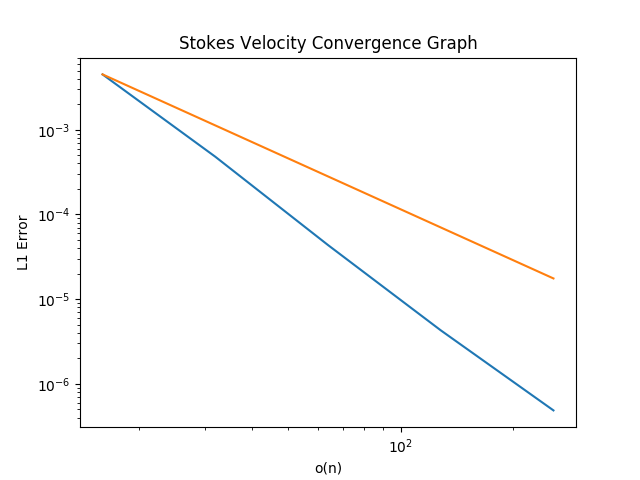
\includegraphics[width=\linewidth]{stokes_convergence_dbc0.png}
  \caption{DG1-BDM2 Stokes velocity convergence plot of velocity error against resolution. The blue curve indicates velocity error, the orange curve is a line of slope $-2$.  We expected order 2 convergence and obtained order 3 convergence. The super convergence is likely due to the symmetric nature of the test solution and the regular mesh.}
\end{figure}

\begin{figure}
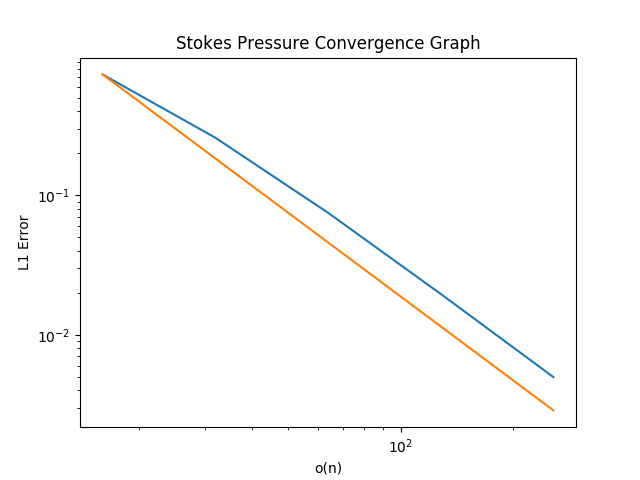
\includegraphics[width=\linewidth]{stokes_pressure_convergence_dbc0.png}
  \caption{DG1-BDM2 Stokes pressure convergence plot of pressure error against resolution. The blue curve indicates pressure error, the orange curve is a line of slope $-2$.  Initially at low orders of $N$ the convergence is not exactly order 2. However as $N$ grows, the order of convergence clearly is 2, indicating that this was just an anomaly due to low resolution.}
\end{figure}



\subsection{Navier-Stokes Convergence}

We again use a manufactured solution to determine the convergence rate of our solver.
We can re-use the manufactured solution in the Stokes convergence test, $u_x = \sin(2 \pi y)^5 \cos(2 \pi y)\sin(2 \pi x)^6$, $u_y= -\sin(2 \pi x)^5 \cos(2 \pi x) \sin(2 \pi y)^6$ and $p = \sin(2 \pi x)^2 \sin(2 \pi y)^2$.\\
However the forcing term will be adjusted. One can find that it will be equivalent to $F = \nabla p - \mu \nabla^2 u + u \cdot \nabla u$.
Plugging this into the equations we find that these do indeed solve the Navier-Stokes equations.\\
Figures 6 and 7 show us the convergence graphs in velocity and pressure.\\
We notice that initially we have the same behavior as in the Stokes case. However we then see the error stopes decreasing. The cause of this is as of yet unknown and would require further research. We did note that changing the test solution and adjusting forcing we always obtain the same pressure error pattern, see figure 8. Additionally note that the pressure solution obtained in all cases respected the implied pressure boundary conditions, suggesting that this is not the problem.

\begin{figure}
  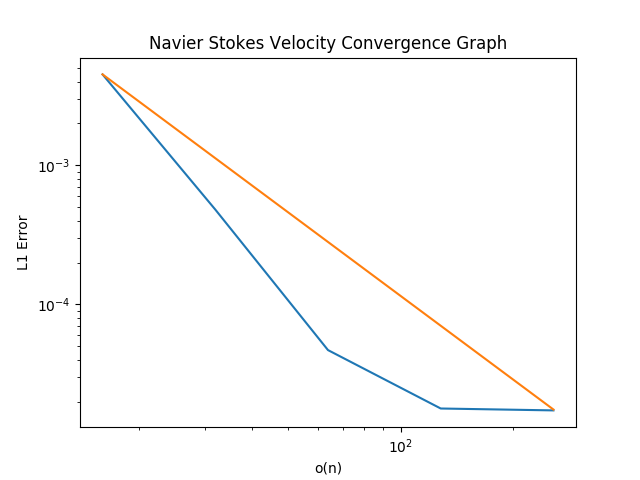
\includegraphics[width=\linewidth]{navier_stokes_convergence_dbc0.png}
  \caption{DG1-BDM2 Navier-Stokes velocity convergence plot of velocity error against resolution.  The blue curve indicates velocity error, the orange curve is a line of slope $-2$.  The velocity error decreases with a logarithmic slope of roughly 2, indicating order 2 convergence, up to $10^{-5}$. The cause for the minimal error has not been found. sWe used the direct solver, not applying the continuation solver.}
\end{figure}

\begin{figure}
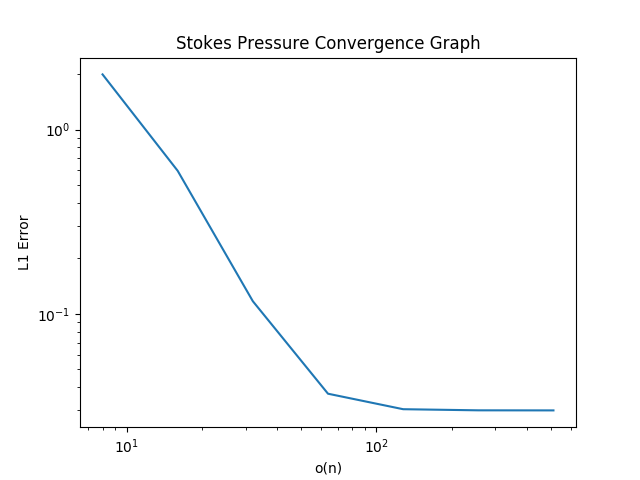
\includegraphics[width=\linewidth]{navier_stokes_pressure_convergence_dbc0.png}
  \caption{DG1-BDM2 Stokes pressure convergence plot of pressure error against resolution. The blue curve indicates pressure error, the orange curve is a line of slope $-2$. The convergence graph here has three phases. Similarly to the Stokes cases, we initially have a lower order convergence due to low number of triangles. Then we have a slope of $2$ as expected. Lastly we have a minimal error, which, as for the velocity, has an unknown cause and thus requires further study. We used the direct solver, not applying the continuation solver.}
\end{figure}

\begin{figure}
  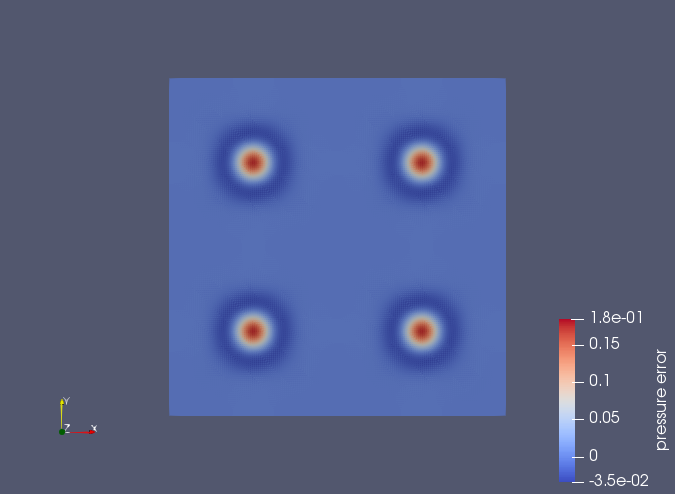
\includegraphics[width=\linewidth]{ns_fail_exp.png}
  \caption{Pressure error using the modified base pressure, $p = x \sin(2 \pi x)^2 \sin(2 \pi y)^2$, and adjusting forcing accordingly. This pattern seems to be repeated regardless of $p$ or $u$ in our tests provided boundary conditions remain the same (in all cases they are $0$).}
\end{figure}

\subsection{Flow Past a Cylinder}

The flow past a cylinder is a well-known and studied flow with interesting properties, such as a change of stability of its steady solution at high Reynolds number.
Our solver still converges to an acceptable error for the velocity fields in this problem.
We will see how our solver resolves this flow to study if we can find unstable solutions and how effective our continuation method is.\\
\\
Figure 9 shows the stokes velocity solution to the problem.\\
Similarly figures 10, 11 and 12 show the velocity solution with full advection at Reynolds numbers $Re = 50$, $25$, and $1$ respectively.\\
We reduce the Reynolds number by reducing the viscosity. As expected this makes the boundary layer about the cylinder smaller and smaller.\\
At higher Reynolds numbers our solver starts requiring to use the continuation method multiple times (by default it always first finds the Stokes solution). For instance we required to find the solution at $0 \%$, $25 \%$, $62.5\%$ and $100\%$ advection for $Re =62.5$, while we only required to find the solution at $0 \%$ and $100 \%$ advection for $Re = 1$.\\
When setting a high Reynolds number, such as $Re = 500$, the solver fails.
\begin{lstlisting}
Reynolds Number =
500.0
Advection term is at 100%
An Exception of type ConvergenceError has occurred. Reducing Step Size.
Advection term is at 50.0%
An Exception of type ConvergenceError has occurred. Reducing Step Size.
Advection term is at 25.0%
An Exception of type ConvergenceError has occurred. Reducing Step Size.
Advection term is at 12.5%
An Exception of type ConvergenceError has occurred. Reducing Step Size.
Advection term is at 6.25%
An Exception of type ConvergenceError has occurred. Reducing Step Size.
Advection term is at 3.125%
An Exception of type ConvergenceError has occurred. Reducing Step Size.
Advection term is at 1.5625%
An Exception of type ConvergenceError has occurred. Reducing Step Size.
Advection term is at 0.78125%
An Exception of type ConvergenceError has occurred. Reducing Step Size.
Advection term is at 0.390625%
An Exception of type ConvergenceError has occurred. Reducing Step Size.
Advection term is at 0.1953125%
An Exception of type ConvergenceError has occurred. Reducing Step Size.
Too low step size, solver failed
\end{lstlisting}
The above output displays when we try this test. We can see the continuation method attempting to solve the problem but failing eventually due too low step-size.\\
According to [14] $Re = 50$ corresponds to the Reynolds numbers where the solution becomes unstable, suggesting that we can find unstable solutions and thus the failure described is not due to instability of our solution.\\
As we performed our tests, we obtained that on a mesh of average triangle edge length $0.5$ with $Re = 48$ we fail in the same manner as for $Re = 500$ for average triangle edge length $0.2$. We can deduce two things from this. First, it is likely that increasing the accuracy of the mesh would allow the solver to work even on high Reynolds number. Second, given that the continuation method is required even though it should only be called when the solver fails to converge within parameters, we can deduce that our continuation method allows us to extend the solvable Reynolds numbers for a given mesh accuracy. Depending on interpretation and available resources this means our continuation method either extends solvable domains or improves speed.

\begin{figure}
  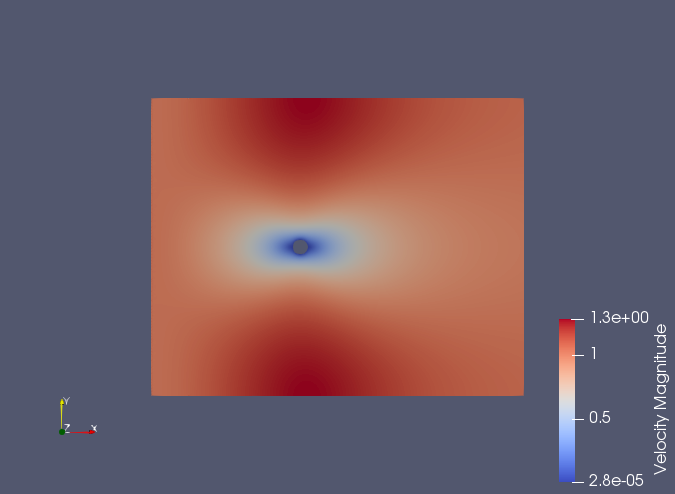
\includegraphics[width=\linewidth]{scR50.png}
  \caption{Stokes flow past a cylinder obtained by the BDM2-DG1 solver. The mesh used has an average triangle edge length of $0.2$ in this figure. We set $\mu = 0.02$, so this also corresponds to the first solution obtained in the $Re =50$ Navier-Stokes solver. Pressure is $0$, and thus does not figure here.}
\end{figure}

\begin{figure}
  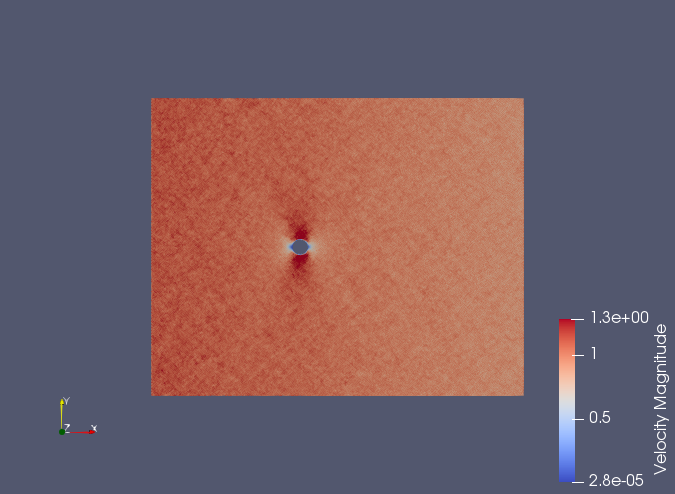
\includegraphics[width=\linewidth]{nscR50.png}
  \caption{Navier-Stokes flow past a cylinder for $Re = 50$ obtained by the BDM2-DG1 solver. The mesh used has an average triangle edge length of $0.2$ in this figure. Notice that the boundary layer is getting smaller as $Re$ increases. Pressure is $0$, and thus does not figure here.}
\end{figure}

\begin{figure}
  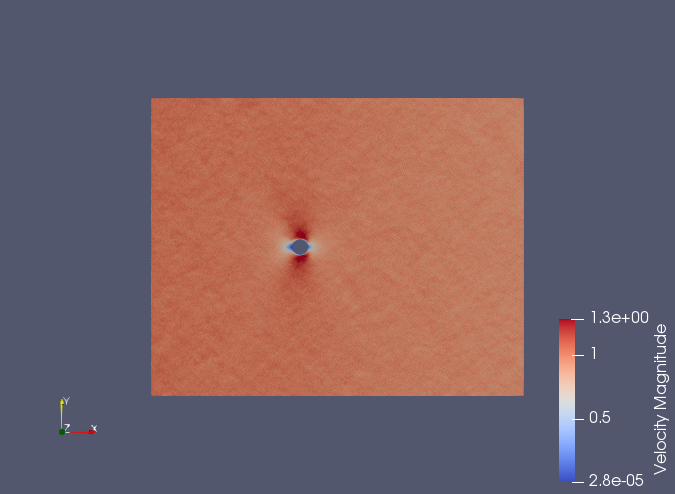
\includegraphics[width=\linewidth]{nscR25.png}
  \caption{Navier-Stokes flow past a cylinder for $Re = 25$ obtained by the BDM2-DG1 solver. The mesh used has an average triangle edge length of $0.2$ in this figure. Notice that the boundary layer is getting smaller as $Re$ increases. Pressure is $0$, and thus does not figure here.}
\end{figure}

\begin{figure}
  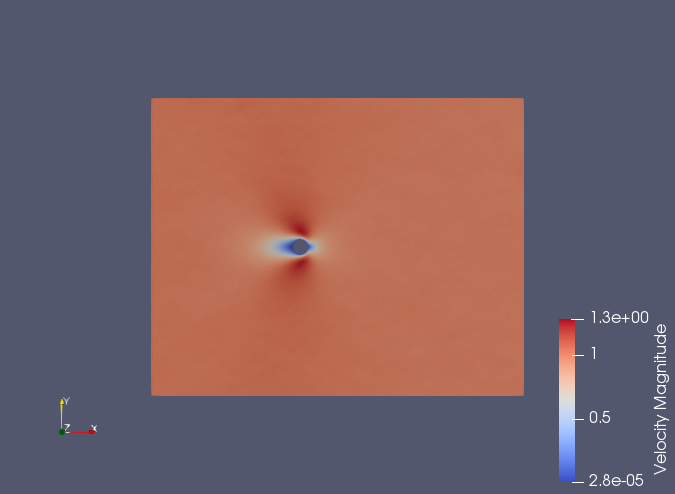
\includegraphics[width=\linewidth]{nscR1.png}
  \caption{Navier-Stokes flow past a cylinder for $Re = 1$ obtained by the BDM2-DG1 solver. The mesh used has an average triangle edge length of $0.2$ in this figure. Notice that the boundary layer is getting smaller as $Re$ increases. Pressure is $0$, and thus does not figure here.}
\end{figure}



\section{Conclusion and Future Improvements}

In this project we were interested in applications of the BDM/DG mixed finite element solver using a modified Schur preconditioner onto the steady Stokes and Navier-Stokes equations.\\
After briefly discussing the general finite element method and some introductory definitions and notations we decided to focus on the Stokes equation. After assembling the weak form of the equation we then applied a Schur preconditioner to improve efficiency.\\
We then assembled a weak form of the Navier-Stokes equation but noted that directly using it was not optimal. As such we developed a continuation method with variable step-size to improve the algorithm's speed and expand the number of problems which it can solve.\\
After this we described a rudimentary time-stepping method to study the stability of any solutions obtained.\\
Finally we tested our steady solvers and concluded that our algorithms worked as anticipated and accomplished our objectives with the exception that the Navier-Stokes error seems to have a lower bound.\\
\\
\\
A number of future improvements could be made.
These would allow us to reduce computational cost and increase the versatility and accuracy of our method.\\
\\
The cause of the lower bound of the Navier-Stokes solver should be found and removed, if possible.\\
We could use a multigrid method using our solver as a smoother to get convergence to be less dependent on grid-size, dramatically reducing computational costs. Application of such a method was discussed, unfortunately the tools required for it are not currently compatible with our problem set (specifically Dirichelet boundary conditions).\\
The variable step-size method is serviceable and can be considerably improved to reduce the total number of iterations and thus computational cost. There are a number of methods which, from local conditions of the function, could more efficiently determine an appropriate step-size. Our source on the continuation method [17] includes descriptions of potential improvements.\\
Similarly the time-stepping method mentioned was designed exclusively for the stability test. For this purpose it would work very well. However various improvements could be made for accuracy and speed. For instance we initially attempted to utilize a Newton iteration rather than a Picards iteration. However as the initial guess was not in the ball of convergence this method failed. Adding a few Newton iterations using the Picard results as a starting point should give more accurate answers for time-dependent methods.\\
The stability test itself could be expanded. For instance we might want to find the growth rate of an instability. Additionally we could also find not only the most unstable mode but all unstable modes by "substracting" unstable modes once they have been determined.\\
In some flows we may have multiple solutions or a bifurcation (that is the case for the cylinder flow at high Reynolds number). In this case a deflation method may be useful. In this method, after finding a solution, we "substract" it from the equation and thus seek other solutions.\\
\\


\section{Appendix}
\subsection{Code}
A significant part of this project was developing a python code using Firedrake.
Firedrake is a python project which aims to provide mathematicians, engineers and scientists with an automated system for solving partial differential equations.\\
It does so by automatically generating code based on UFL expressions from the FEniCS project, a library of computational methods used for solving PDEs. This allows us to write out our equations in a fairly intuitive way while Firedrake generates the background code needed to solve them.\\
Our project comprises largely of one file containing the rinsp and rinspt classes, though various launching scripts and the Lagrange script are also present. We will not discuss the entirety of either class, if the reader wants to have a detailed look he can go to the github repository containing them at https://github.com/Frostyant/M4R\_Navier\_Stokes\_Solvers once it has been made public.\\
We will however show a handful of code snippets, ranging from the parameters firedrake uses to generate the code to the UFL expressions for the advection terms. This will explain some of the computational practical aspects and demonstrate exactly how we used Firedrake, UFL and FEniCS.

\subsubsection{Solver Paremeters}
The parameters of our solver are :
\begin{lstlisting}
"ksp_type": "gmres",
            "ksp_converged_reason": True,
            "ksp_rtol": 1e-6,
            "ksp_max_it": 50,
            "pc_type": "fieldsplit",
            "pc_fieldsplit_type": "schur", #use Schur preconditioner
            "pc_fieldsplit_schur_fact_type": "full", #full preconditioner
            "pc_fieldsplit_off_diag_use_amat": True,
            "fieldsplit_0_ksp_type": "preonly",
            "fieldsplit_0_pc_type": "lu",#use full LU factorization, ilu fails
            "fieldsplit_0_pc_factor_mat_solver_type": "mumps",
            "fieldsplit_1_ksp_type": "preonly",
            "fieldsplit_1_pc_type": "bjacobi",
            "fieldsplit_1_pc_sub_type": "ilu"#use incomplete LU factorization on the submatrix
\end{lstlisting}
GMRES indicates the solver used for the outer system.
 It stands for generalized minimal residual method, and used due to nonsymmetric nature of our equation.\\
ksp\_rtol indicates the relative tolerance above which we consider that the equation diverges.\\
ksp\_max\_it is the maximal number of iterations for the linear GMRES solver. If above the maximal number of iterations, the solver fails or, in the continuation method, reduces $c$ in the advection term and tries again.\\
"pc\_type": "fieldsplit" tells the algorithm that the matrix has a block structure as describe in the Schur preconditioner section.\\
"pc\_fieldsplit\_type": "schur" indicates we are using the Schur fieldsplit preconditioner.\\
"pc\_fieldsplit\_off\_diag\_use\_amat": True indicates that the offdiagonal terms, ie the $B$ and $B^T$ described in section 4.1.2, whould be taken from the original matrix directly. \\
"fieldsplit\_0 options deal with finding $A^{-1}$ in the Schur Preconditioner while the fieldsplit\_1 options deal with the remaining part of the preconditioner.\\
 "fieldsplit\_1\_pc\_sub\_type": "ilu is how we indicate the direct inversion of the block diagonal pressure-mass matrix approximating $S$.

\subsubsection{Advection Term}
The UFL plugin allows us to write out our weak equations almost directly into code. Pieces of code can thus be deduced directly from the weak forms determined in sections 4.1.1, 4.2.1 and 4.3.1. We show the advection term here, both to display an example as well as to discuss some specifics when dealing with 2D problems.\\
The code associated to the advection term is :
\begin{lstlisting}
def GetAdvectionTerm(self,up,InflowBc,Bcs):

        n = FacetNormal(self.mesh)
        #splitting u and p for programming purposes (unavoidable)
        u, p = split(up)

        #Re-Defining functions for use in Advection term
        if self.twoD:
            curl = lambda phi: as_vector([-phi.dx(1), phi.dx(0)])
            cross = lambda u, w: -u[1]*w[0]+u[0]*w[1]
            perp = lambda n, phi: as_vector([n[1]*phi, -n[0]*phi])
        else:
            perp = cross

        #Defining upwind and U_upwind for use in advection
        Upwind = 0.5*(sign(dot(u, n))+1)
        U_upwind = Upwind('+')*u('+') + Upwind('-')*u('-')

        #Assembling Advection Term
        adv_byparts1 = inner(u, curl(cross(u, self.v)))*dx
	#This is the term from integration by parts of double curl
        adv_byparts2 = inner(U_upwind, 2*avg( perp(n, cross(u, self.v))))*dS
	#Second term over surface
        adv_grad_parts1 = 0.5*div(self.v)*inner(u,u)*dx
	#This is the term due to the integration by parts of grad u^2
        if not InflowBc:
            adv_bdc1 = inner(u,perp(n,cross(u,self.v)))*ds(Bcs)
	#boundary version of adv_byparts2
            adv_grad_parts2 = 1/2*inner(inner(u,u)*self.v,n)*ds(Bcs)
	#boundary term from grad u^2 integration by parts
        else:
            adv_bdc1 = inner(u,perp(n,cross(u,self.v)))*ds(Bcs)
	#boundary version of adv_byparts2
            adv_grad_parts2 = 1/2*inner(inner(u,u)*self.v,n)*ds(Bcs)
	#boundary term from grad u^2 integration by parts
            adv_bdc1 +=  inner(self.u_0,perp(n,cross(self.u_0,self.v)))*ds(InflowBc)
	#boundary version of adv_byparts2
            adv_grad_parts2 += 1/2*inner(inner(self.u_0,self.u_0)*self.v,n)*ds(InflowBc)
	#boundary term from grad u^2 integration by parts

        advection_term = (
            adv_byparts1
            - adv_byparts2
            - adv_grad_parts1
            - adv_bdc1
            + adv_grad_parts2
        )

        return advection_term
\end{lstlisting}
Note that inflow boundary conditions have to be treated separately from no-slip boundary conditions.\\
Additionally note that we had to specify a special case for 2D. While most of the UFL code works in 2D and 3D in the same way, the cross product is ill-defined purely in 2D. Hence we needed to define special operations for each possible instance of the cross product.\\

\subsection{Selecting the Manufactured Solution}
We will now introduce the method of manufactured solution, which we used multiple times to determine the accuracy and rate of convergence of the various computational methods discussed. While the method is simple, it primarily involves artificially creating a solution to the equation by adjusting the forcing term and boundary conditions, some thought has to be put into selecting the solution. Otherwise we may find that the algorithms do not converge.\\
Firstly any manufactured solution needs to actually solve the equations. For simplicity we eliminate the continuity equation by considering the stream function rather than the velocity field. Where the stream function is defined is :
\begin{align*}
\frac{ \partial \psi}{\partial y} = u_x \\
-\frac{\partial \psi}{\partial x} = u_y
\end{align*}
When selecting the manufactured solution we want one which is preferably as simple as possible and easy to check. For instance we had $0$ boundary conditions in velocity. This both made determining errors on the boundaries easy and avoided a lot of the issues that come with outflows and inflows for the Navier-Stokes equations. For the streamfunction this implies that the derivatives are 0 at the boundaries. We can easily resolve this by setting $\psi = \sin(2 \pi x)^n \sin(2 \pi y)^n$ with n greater than 2.\\
Another thing to consider is the pressure boundary conditions. We technically did not force any, but the equation naturally has them. Consider dotting the Navier-Stokes equations with the normal at the boundaries.
\begin{align*}
\nabla p \cdot n &= -(u \cdot \nabla) u \cdot n  + \mu \nabla^2 u \cdot n + F \cdot n, \\
x \in \delta \Omega,
\end{align*}
where we evaluate the entire equation at x, a point on the boundary.
Thus the normal Dirichelet velocity boundary conditions imply boundary conditions on $\frac{\partial p}{\partial n}$.\\
For simplicity we want this to be $0$ too.\\
Note how every term on the left-hand side is either proportional to $\psi$, one of its derivatives or a sum of those. Hence all these terms become $0$ at all the boundaries if $n$ is large enough (as we would have $ \sin(2 \pi x) \sin(2 \pi y)$ terms).\\
This can be verified, as when failing to get a large enough $n$ and attempting to solve for the $0$ pressure solution we will get a trigonometric structure on the boundaries in the pressure error as seen in figure 13.\\
As for setting the pressure, we need to ensure that $\frac{\partial p} {\partial n} = 0$, using a similar method to above we can consider $p =  \sin(2 \pi x)^2 \sin(2 \pi y)^2$.\\
Hence we get our standard manufactured solution :
\begin{align}
u_x = \sin(2 \pi y)^5 \cos(2 \pi y)\sin(2 \pi x)^6 \\
u_y= -\sin(2 \pi x)^5 \cos(2 \pi x) \sin(2 \pi y)^6 \\
p = \sin(2 \pi x)^2 \sin(2 \pi y)^2
\end{align}

\begin{figure}
  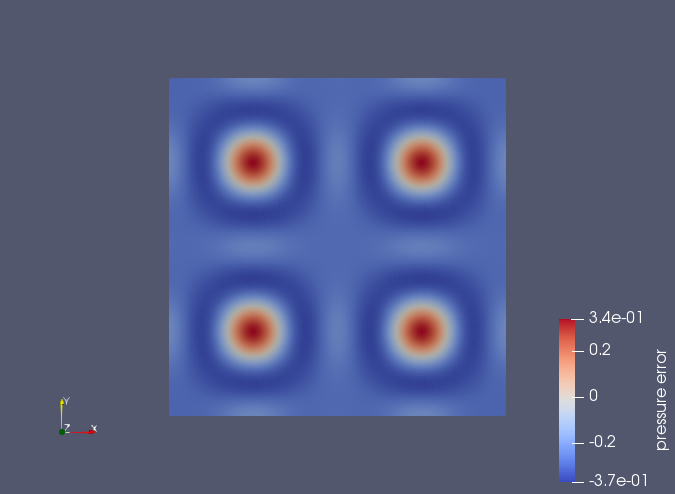
\includegraphics[width=\linewidth]{badpbdc.png}
  \caption{Pressure error of the Navier-Stokes equation when $n$ in $\psi = \sin(2 \pi x)^n \sin(2 \pi y)^n$  is equal to 2. Notice that the error is a combination of $\sin$ and $\cos$ on the boundary. The form of $\psi$ implies non-zero Neumann boundary conditions in pressure in a trigonometric form (ie a combination of $\sin$  and $\cos$).}
\end{figure}

\section{Citations}

[1] Imperial College London \textit{Firedrake Project} Available from :\\
 https://www.firedrakeproject.org [Accessed throughout 2018-2019]\\

[2] Patrick E. Farrell, Lawrence Mitchell, Florian Wechsung
textit{ An Augmented Lagrangian Preconditioner For The 3D Stationary Incompressible Navier–Stokes Equation At High Reynolds Number}
SIAM J. Sci Comput 28(6)2006\\

[3] Arnold, Douglas N., et al. \textit{Unified analysis of discontinuous Galerkin methods for elliptic problems.} SIAM journal on numerical analysis 39.5 (2002): 1749-1779.\\

[4] Vassilevski, Panayot S. \textit{Multilevel Block Factorization Preconditioners: Matrix-based Analysis and Algorithms for Solving Finite Element Equations.} New York, NY: Springer New York, 2008. Web.\\

[5] Ibrahimbegovic, Adnan. \textit{Nonlinear Solid Mechanics}. Vol. 160. Dordrecht: Springer Netherlands, 2009. Solid Mechanics and Its Applications. Web.\\

[6] Thomée, Vidar. (1986). \textit{Galerkin finite element methods for parabolic problems}. SERBIULA (sistema Librum 2.0). 25. 10.1007/978-3-662-03359-3. \\

[7]  Kirby R.C., Logg A., Rognes M.E., Terrel A.R. (2012) \textit{Common and unusual finite elements}. In: Logg A., Mardal KA., Wells G. (eds) Automated Solution of Differential Equations by the Finite Element Method. Lecture Notes in Computational Science and Engineering, vol 84. Springer, Berlin, Heidelberg\\

[8] Hansbo, Peter \& Larson, Mats. (2003). \textit{Discontinuous Galerkin and the Crouzeix–Raviart element: Application to elasticity}. \\
http://dx.doi.org/10.1051/m2an:2003020. 37. 10.1051/m2an:2003020. \\

[9] Olshanskii, Maxim \& Reusken, Arnold. (2004). \textit{Grad-div stabilization for Stokes equations}. Mathematics of Computation - Math. Comput.. 73. 1699-1718. \\

[10] Huan Zhengda, \textit{The convergence ball of Newton's method and the uniqueness ball of equations under Hölder-type continuous derivatives},
Computers \& Mathematics with Applications,
Volume 47, Issues 2–3,
2004,
Pages 247-251,
ISSN 0898-1221,
https://doi.org/10.1016/S0898-1221(04)90021-1.\\

[11] X Wang, \textit{Convergence of Newton's method and uniqueness of the solution of equations in Banach space}, IMA Journal of Numerical Analysis, Volume 20, Issue 1, January 2000, Pages 123–134,\\
 https://doi.org/10.1093/imanum/20.1.123\\

[12] Bae, Jong Sook, and Sangsuk Yie. \textit{Range of Gateaux Differentiable Operators and Local Expansions}  Pacific J. Math. 125.2 (1986): 289-300. Web.\\

[13] Zi-Cai Li, Cheng-Sheng Chien, Hung-Tsai Huang,\textit{
Effective condition number for finite difference method},
Journal of Computational and Applied Mathematics,
Volume 198, Issue 1,
2007,
Pages 208-235,
ISSN 0377-0427,
https://doi.org/10.1016/j.cam.2005.11.037.\\

[14] Hashiguchi, Masanori \& Kuwahara, Kunio. (1996). \textit{Two-Dimensional Study of Flow past a Circular Cylinder}. RIMS Kokyuroku. 974. \\

[15] Cockburn B, Kanschat G, Schötzau D. \textit{A note on discontinuous galerkin divergence-free solutions of the navier-stokes equations. Journal of Scientific Computing}. 2007 Jun 1;31(1-2):61-73. https://doi.org/10.1007/s10915-006-9107-7\\

[16] Constantinescu V.N. (1995) \textit{Other Solutions of Navier-Stokes Equations (Steady Incompressible Flow).} In: Laminar Viscous Flow. Mechanical Engineering Series. Springer, New York, NY\\

[17] Deuflhard P. (2011) Parameter Dependent Systems: Continuation Methods. In: \textit{Newton Methods for Nonlinear Problems}. Springer Series in Computational Mathematics, vol 35. Springer, Berlin, Heidelberg\\

[18] Natale, Andrea, and Colin J. Cotter. \textit{Scale‐selective Dissipation in Energy‐conserving Finite‐element Schemes for Two‐dimensional Turbulence}  Quarterly Journal of the Royal Meteorological Society 143.705 (2017): 1734-745. Web.\\

[19] Paniconi, C., and Putti, M. ( 1994), \textit{A comparison of Picard and Newton iteration in the numerical solution of multidimensional variably saturated flow problems}, Water Resour. Res., 30( 12), 3357– 3374, doi:10.1029/94WR02046.\\

[20] Hui Xu, Yinnian He,
\textit{Some iterative finite element methods for steady Navier–Stokes equations with different viscosities},
Journal of Computational Physics,
Volume 232, Issue 1,
2013,
Pages 136-152,
ISSN 0021-9991,\\
https://doi.org/10.1016/j.jcp.2012.07.020.\\
(http://www.sciencedirect.com/science/article/pii/S0021999112003932)\\

[21] Utku, and Carey. \textit{Boundary Penalty Techniques.} Computer Methods in Applied Mechanics and Engineering 30.1 (1982): 103-18. Web. \\

[22] Dai, Xiaoxia. \textit{Finite Element Approximation of the Pure Neumann Problem Using the Iterative Penalty Method.} Applied Mathematics and Computation 186.2 (2007): 1367-373. Web.\\



\end{document}
